\documentclass[11pt]{article}
\usepackage[utf8]{inputenc}
\usepackage[labelfont=bf]{caption}
\usepackage[compact]{titlesec}
\usepackage{appendix}
\usepackage{graphicx,amsmath,booktabs,subcaption,placeins,mathtools,multirow} % All of the classics
\usepackage{tikz}
\usepackage[activate={true,nocompatibility},
    final,
    tracking=true,
    kerning=true,
    spacing=true,
    factor=1100,
    stretch=10,
    shrink=10]{microtype}
    \microtypecontext{spacing=nonfrench}
\usepackage[colorlinks,
    linkcolor=teal,
    citecolor=teal,
    filecolor=teal,
    urlcolor=teal]{hyperref}
\usepackage[margin=1in]{geometry} % 1in margins
\usepackage[version=4]{mhchem}

\DeclareCaptionLabelFormat{withincaption}{#2)}
\captionsetup{subrefformat=withincaption}

% -- Use the Charter fonts as base fonts, fixup math-mode display
\usepackage[charter]{mathdesign}
\usepackage[scaled=.96,osf]{XCharter}
\linespread{1.04}
\usepackage[backend=biber,style=nature,backref=true]{biblatex} %author-year for in-text content
%\hyphenpenalty=750
\usepackage{cleveref}
%-------------------end standard preamble-------------------------
\newcommand{\units}[2]{\frac{\text{#1}}{\text{#2}}\,}
\newcommand{\unit}[1]{\; \text{#1}\,}

\titlespacing{\section}{0pt}{2ex}{1ex}
\titleformat{\subsection}[display]{\bfseries}{}{0em}{}
\titlespacing{\subsection}{0pt}{0.1em}{0.1em}

\title{TANGLES: modeling supercoiling-dependent feedback\\DNA supercoiling coordinates transcription via topologically-active networks of genes }
\author{Christopher P. Johnstone, Kate E. Galloway}
\date{ }

\addbibresource{main_library.bib}

\begin{document}
\maketitle

\section{Introduction}
Cells coordinate complex behaviors through precise spatiotemporal control of gene expression. To rapidly advance the power of gene- and cell-based therapies, synthetic biology aims to harness the power of native biology by constructing synthetic gene regulatory networks capable of dynamically prescribing cellular processes, states, and identities.\parencite{chenSyntheticBiologyAdvancing2012,beitzSyntheticGeneCircuits2022,purnickSecondWaveSynthetic2009,elowitzBuildLifeUnderstand2010}
Synthetic networks process diverse inputs into complex logical and temporal responses.\parencite{weinbergLargescaleDesignRobust2017,xieMultiInputRNAiBasedLogic2011,taborSyntheticGeneticEdge2009}
From oscillators to pulse generators, synthetic circuits can  precisely coordinate dynamic patterns of gene expression across populations of cells to control cell fate.\parencite{gardnerConstructionGeneticToggle2000,elowitzSyntheticOscillatoryNetwork2000,strickerFastRobustTunable2008,daninoSynchronizedQuorumGenetic2010,maSyntheticMammalianSignaling2020a,parkEngineeringEpigeneticRegulation2019,bashorUsingEngineeredScaffold2008,gallowayDynamicallyReshapingSignaling2013}
However, rational de novo design of synthetic circuits remains challenging. Despite extensive biomolecular modeling, integration of single genetic elements into systems often leads to emergent behaviors, requiring iterative design-build-test cycles to achieve the desired performance.\parencite{jonesEndoribonucleasebasedFeedforwardController2020,freiCharacterizationMitigationGene2020,qianResourceCompetitionShapes2017}
Compounding the challenge, transcription exhibits significant extrinsic and intrinsic noise.\parencite{toNoiseCanInduce2010,zopfCellCycleDependenceTranscription2013,desaiDNArepairPathwayCan2021}
In particular, the stochastic nature of transcription makes coordinating expression across multiple genetic elements challenging.\parencite{rodriguezIntrinsicDynamicsHuman2019,rodriguezTranscriptionLivingCells2020,quartonUncouplingGeneExpression2020}
Spatial variation in the nucleus and biochemical dynamics in condensates may contribute to bursting but provide limited parameters for tuning transcriptional noise.\parencite{henningerRNAMediatedFeedbackControl2020,guoPolIIPhosphorylation2019}
Alternatively, mechanical sources of gene regulation offer one potential mechanism by which to understand and harness transcriptional noise to improve the predictable design of gene circuits.\parencite{johnstoneEngineeringCellularSymphonies2021,anconaTranscriptionalBurstsNonequilibrium2019a,kimLongDistanceCooperativeAntagonistic2019,elhoudaiguiBacterialGenomeArchitecture2019a,meyerTorsionMediatedInteractionAdjacent2014}.

The mechanical forces of DNA supercoiling powerfully shape transcriptional variance.\parencite{desaiDNArepairPathwayCan2021,chongMechanismTranscriptionalBursting2014}
Chromatin, the DNA polymer wrapped around nucleosomes and decorated with regulatory proteins, regulates diverse processes from transcription to differentiation. With enhanced resolution in the layers and dynamics of chromatin structure, the manifold functions of chromatin-mediated gene regulation are emerging.\parencite{hsiehResolving3DLandscape2020,krietensteinUltrastructuralDetailsMammalian2020}
In the process of transcription, RNA polymerases induce a leading wave of positive DNA supercoiling\parencite{wuTranscriptionGeneratesPositively1988,liuSupercoilingDNATemplate1987}, reshaping the local structure of chromatin.\parencite{acharNegativeSupercoilGene2020,tevesTranscriptiongeneratedTorsionalStress2014a,naughtonTranscriptionFormsRemodels2013,guoHighresolutionGenomewideMapping2021a}
At the kilobase scale, chromatin structure correlates with gene regulation.\parencite{hsiehResolving3DLandscape2020,rowleyEvolutionarilyConservedPrinciples2017}
In yeast and human cells, transcriptionally-induced supercoiling demarks bounds of gene activity.\parencite{acharNegativeSupercoilGene2020,naughtonTranscriptionFormsRemodels2013}
In particular, transcriptional activity dictates the strength of contact domains such as gene-to-gene interactions, indicating a role for transcription in forming and maintaining interactions at the kilobase scale.\parencite{rowleyOrganizationalPrinciples3D2018,rowleyEvolutionarilyConservedPrinciples2017}
Together these data suggest that the process of transcription drives formation of supercoiling-linked, kilobase-scale structures that feedback into transcriptional regulation of gene expression. Biophysical models of gene expression predict that changes in DNA supercoiling in turn change transcriptional activity.\parencite{sevierPropertiesGeneExpression2018}
As supercoiling rapidly diffuses across long distances \parencite{loenhoutDynamicsDNASupercoils2012}, transcriptional activity at one site may impact the overall activity and dynamics of transcription of proximal genes.\parencite{sevierCollectivePolymeraseDynamics2022,tripathiDNASupercoilingmediatedCollective2021}
By understanding how supercoiling induces coupling between neighboring genes provides the opportunity to improve the predictable design of transgenic systems from simple reporters to sophisticated dynamic circuits.

Here we develop a model of transcriptional regulation that integrates DNA supercoiling to examine how the activity of neighboring genes in differing orientations affects expression of both genes.
(We need to define what models that exist already…what they found for context of what is currently predicted and highlight gaps (that our model will fill). Their models focus on RNA polymerase speed which seems to be a difficult to measure experimental feature. I will be looking at these models more closely to highlight differences. Please feel free to add here as well.)
(1-3 sentences of our model description; this can be integrated with above to juxtapose choices).
We find….(summary of figure 1 and 2)
We extend this model to examine a synthetic toggle switch composed in different orientations to predict the effect of DNA supercoiling on the stability of states, examine transition dynamics, and define the critical parameters for designs in different orientations. We find…(summary of figure 3)
Further, we adapt our model to investigate the explanatory power of DNA supercoiling as a mechanism for coordinating expression between divergently expressed genes in the drosophila segmentation network. We find …(summary of figure 4)
Finally, to examine how our toggle switch behavior will vary across cells with varying topoisomerase expression, we investigate the sensitivity of the toggle switch to varying topoisomerase activity. We find……(summary of figure 5; we might want to switch the order of fig 4 and 5)

\begin{figure}[h]
    \centering
    \caption{Graphical abstract} \label{fig:graphical_abstract}
\end{figure}

\section{Model and methods}
Simulating the behavior of native and synthetic circuits under the influence of transcription-induced feedback requires an model that integrates explicitly-modeled polymerase motion and RNA- and protein-mediated feedback mechanisms.
Our method combines three modeling levels: an ordinary differential equation model that simulates the continuous progression of polymerases loaded onto DNA, a core stochastic model that models supercoiling-dependent polymerase initiation, and a user-specified stochastic layer that allows for modeling of other regulatory interactions such as the promoter-repressive and -activating interactions used in synthetic circuits.

\subsection{Continuous model of supercoiling-dependent transcription}
Here, supercoiling is defined as the amount of excess twist \(\phi\) relative to relaxed DNA (with relaxed DNA having twist \(\omega_0 = 1.85\) radians/nm, or 1 full revolution per \(\approx10\) basepairs). While the supercoiling density could more generally be defined as a varying function of genomic location \(\sigma(z)\), in a region of constant supercoiling density, we can use the excess twist at the endpoints \(z_1, z_2\) to define the supercoiling density as:
\begin{equation}
    \sigma = \frac{\phi(z_1) - \phi(z_2)}{\omega_0 (z_2 - z_1)}
\label{eq:supercoiling_density}
\end{equation}
Note that \cref{eq:supercoiling_density} is defined such that a positive value of \(\phi\) at an intermediate point between two endpoints with \(\phi=0\) (relaxed DNA) means that the supercoiling density is \emph{positive} in front of the intermediate point and \emph{negative} behind the intermediate point. Following on the work of \textcite{sevierPropertiesGeneExpression2018}, we assume that on the length scales of synthetic and native circuits of interest (\(O(\approx10kb)\)), the supercoiling density is constant in all regions between polymerases and other barriers. Because supercoiling diffusion and plectoneme hopping \parencite{loenhoutDynamicsDNASupercoils2012} occur at a faster rate (diffusion constant of \(\mathcal{D} \approx O(0.5 \units{kb$^2$}{s})\)) than transcription (\(v_0 \approx 50 \units{bp}{s}\)) \parencite{munizRNAPolymeraseII2021}, the assumption of supercoiling relaxation on the timescale of transcription simplifies the resulting model.

How does transcription both drive the process of supercoiling generation and react to changes in local supercoiling? Under the assumption of supercoiling relaxation, each polymerase is defined by four variables--the (one-dimensional) genomic location of the polymerase \(z_i\), the length of the nascent RNA \(x_i\), the excess twist at the location of the polymerase \(\phi_i\), and the rotation angle of the polymerase \(\theta_i\). Then, two governing equations define the motion of all polymerases. The first equates the linear motion of the polymerase with the rotational motion (either of the RNAP or of the DNA) required for the polymerase to track the DNA groove,
\begin{equation}
    \underbrace{\omega_0 \frac{dz_i}{dt}}_{\mathclap{\text{RNAP velocity}}} = \overbrace{\frac{d\theta_i}{dt}}^{\mathclap{\text{RNAP rotation}}} + \underbrace{\frac{d\phi_i}{dt}}_{\mathclap{\text{supercoiling generation}}}
\label{eq:linear_rotational_balance}
\end{equation}
whereas the second is a torque balance between the DNA-mediated torques and
\begin{equation}
    \underbrace{\tau(\sigma(z_i, \phi_{i-1}, \phi_{i+1}))}_{\mathclap{\text{torque acting on RNAP}}} + \overbrace{\chi \frac{d\phi_i}{dt}}^{\mathclap{\text{supercoiling restoring force}}}= \underbrace{\eta x_i^n \frac{d\theta_i}{dt}}_{\mathclap{\text{nascent RNA drag}}}
\label{eq:torque_balance}
\end{equation}
\Cref{eq:linear_rotational_balance,eq:torque_balance} can be solved as in \textcite{sevierPropertiesGeneExpression2018} to give a set of ordinary differential equations as long as we define equations for the torque response \(\tau(\sigma)\) as a function of the local supercoiling density and the RNAP velocity as a function of local torque \(\frac{dz}{dt} = v(\tau)\). Here, we use Marko's torque-response model to supercoiling which accounts for the thermodynamic behavior of both non-buckled, twisted DNA and buckled, plectonemic DNA \parencite{markoTorqueDynamicsLinking2007}. The resulting \(\tau(\sigma)\) functions exhibits a phase transition, where the torque response is nearly constant at intermediate values of \(\sigma\) where the DNA is transitioning from a locally-twisted phase to a plectonemic-phase.

For the velocity response of a polymerase experiencing a torque \(\tau_f\) in front and \(\tau_b\) behind, we chose to model polymerase stalling as:
\begin{equation}
    v(\tau_f, \tau_b) = \frac{v_0}{(1 + e^{(|\tau_f| - \tau_s)/\tau_w})(1 + e^{(|\tau_b| - \tau_s)/\tau_w})}
\label{eq:velocity_response}
\end{equation}
where the stall torque \(\tau_s = 12 \unit{pN nm}\) and stall-width \(\tau_w = 3 \unit{pN nm}\) define a sigmoidal stall-response curve.
As shown in \cref{fig:supp_tau_hyperparameter_sweep}, our results are only weakly dependent on the specific choice of \(\tau_s\) and \(\tau_w\).
Importantly, our selected phenomenological term will stall polymerase motion if \emph{either} the torque upstream or downstream exceeds the stall torque \(\tau_s\), in contrast to models such as \textcite{tripathiDNASupercoilingmediatedCollective2021}. We chose this form of the velocity equation because ???\footnote{In any case, our choice is conservative in the sense that it would predict \textbf{more} stalling than Tripathi, yet we see very robust expression/lots of loaded polymerases later. How do I say this nicely here?}


Taking the above equations together, we can simulate the coupled motion of an arbitrary number of polymerases as a single coupled ODE system. We further implemented different boundary conditions, allowing us to simulate both circular topologies, applicable to experimental plasmid systems, and linear topologies, applicable to native or genomically-integrated circuits.

\subsection{Modeling supercoiling-dependent initiation}
With the ability to simulate arbitrary numbers of polymerases, we need a way to model the addition of polymerases to simulated genes. A simple strategy is to assume a supercoiling-independent initiation rate and use a stochastic simulation method to randomly add polymerases to transcriptional start sites at a certain fixed rate. However, this may miss important dynamics. Modeling polymerase initiation as a single-step reaction that proceeds with a certain rate, there is a corresponding energy barrier for polymerase addition. By adding additional supercoiling-dependent energy terms, we can model the extra energy cost for polymerase binding under different local supercoiling conditions. Under the approximation that the direct energetic cost of locally melting the DNA to fit in the RNAP groove dwarfs the relative change in unwinding energy caused by supercoiling, the majority of the energetic cost comes from inserting supercoiling ahead and behind the inserted polymerase. Under this assumption, the first-order supercoiling energetic correction can be written as:
\begin{equation}
    E_\text{sc} = 1.2  \cdot 2\pi \cdot \tau(\sigma)
\label{eq:first_order_sc_initation}
\end{equation}
A full derivation of this result is given in \cref{sec:sc_initation_derivation}. As seen in \cref{fig:including_melting_rnap}, if the approximation that leads to \cref{eq:first_order_sc_initation} is not made, then only minor energetic changes occur.

While this first-order energetic term introduces much-needed behavior to the modeled system, where locally high positive supercoiling decreases the RNAP initiation rate and locally negative supercoiling increases the RNAP initiation rate, at extreme values of \(\sigma\), this energetic term gives unphysical predictions. In particular, under highly negative supercoiling densities, the energetics of polymerase loading becomes increasingly favorable, with loading sometimes occurring more than two orders of magnitude faster when compared to relaxed DNA. To correct for behavior, we added a second-order term of the form that disfavors polymerase loading at highly positive or negative local supercoiling:
\begin{equation}
    E_\text{sc} = 1.2  \cdot 2\pi \cdot \tau(\sigma) + \alpha \cdot \tau_0 \cdot \sigma^2
\label{eq:second_order_sc_initation}
\end{equation}
for \(\tau_0\), the relevant scale factor in the \(\tau(\sigma)\) equation \parencite{markoTorqueDynamicsLinking2007} and \(\alpha\) a positive tunable parameter. As the \(\tau(\sigma)\) equation is linear in \(\sigma\) outside of the phase-transition region, this added \(\sigma^2\) term can be contextualized as an additional term in the Taylor expansion of the physically-realistic \(E_\text{sc}(\sigma)\) equation.

When simulating the ODE model, the rate of stochastic polymerase initiation then varies continuously based on the local supercoiling density \(\sigma\) at the transcription start site as:
\begin{equation}
    r_\text{initation} = r_\text{base rate} e^{- E_\text{sc} / (k_B T)}
\label{eq:intermediate_init_rate}
\end{equation}


\subsection{Modeling additional stochastic, discrete reactions}
Many of the native and synthetic systems of interest include other regulatory species. In order to analyze these types of systems using our supercoiling model, we extended our model to simultaneously simulate arbitrary discrete stochastic equations---such as those commonly used in the literature to model protein production, degradation, dimerization, and more.
In addition, we allowed the base initiation rate of genes to vary as an arbitrary function of all species concentrations (\(\vec s\)) in the model, such that \cref{eq:intermediate_init_rate} becomes:
\begin{equation}
    r_\text{initation} = r(\vec s) e^{- E_\text{sc} / (k_B T)}
\label{eq:final_init_rate}
\end{equation}
For example, a cooperative repressive interaction between some protein species \(s_1\) and a promoter could be modeled using a repressive Hill function:
\[
    r(\vec s) = \frac{r_\text{base}}{1 + \left(\frac{s_1}{K}\right)^n}
\]
When combined with discrete stochastic reactions, we can model a wide range of phenomena. Importantly, we simulated the activity of topoisomerases in this way.

\section{Results}

\subsection{DNA supercoiling dynamics confer rapid, tunable coupling between adjacent genes in varied contexts}
In order to characterize the behavior of supercoiling-mediated feedback, we simulated a series of simple two-gene circuits. In addition to being experimentally accessible, two-gene circuits allow us to test and understand the core design considerations---circuit syntax, relevant boundary conditions, and experimentally tunable model parameters---while still retaining interpretability.
The first major prediction involves the

\begin{itemize}
    \item Supercoiling allows for regulation on timescales otherwise inaccessible by synthetic systems.

    \item (probably we should say something about noise and controlling for it via syntax)

    \item Divergent gene orientation can lead to strongly correlated bursting on short timescales.

    \item Supercoiling-dependent initiation, modeled here as an expansion based on assumptions reasonable for real systems, is a key supercoiling-dependent mechanism that is balanced against polymerase stalling.

    \item Expression context provides different boundary conditions, inducing different levels of supercoiling-dependent feedback.

    \item Regulatory systems involving supercoiling are capable of sense changes in genomic context, such as changes in adjacent gene expression and accessibility.
\end{itemize}


\begin{figure}[h]
    \centering
    {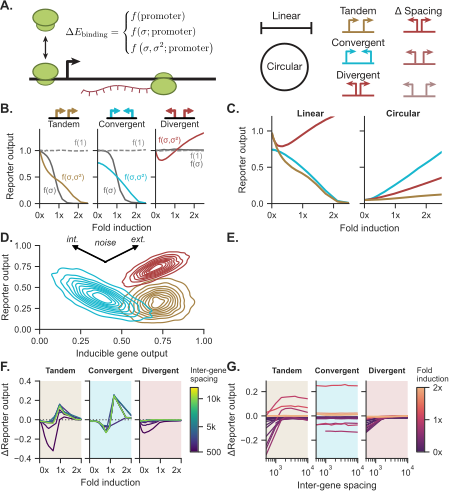
\includegraphics{figures/modeling_paper/fig_1.pdf}
    \phantomsubcaption\label{fig:supercoiling_with_energy_cartoon}
    \phantomsubcaption\label{fig:reporter_output_by_init_type}
    \phantomsubcaption\label{fig:reporter_output_by_bc}
    \phantomsubcaption\label{fig:output_distribution_by_orientation}
    \phantomsubcaption\label{fig:intergene_spacing_cartoon}
    \phantomsubcaption\label{fig:reporter_output_by_intergene_spacing}
    \phantomsubcaption\label{fig:reporter_output_by_spacing_fold_induction}}
    \caption{Supercoiling-dependent polymerase motion and polymerase initiation predict context-dependent circuit behavior.
        \subref{fig:supercoiling_with_energy_cartoon}  Polymerases generate positive and negative supercoiling ahead and behind as they move. Polymerase initiation can be modeled as independent or dependent of the local supercoiling density. A supercoiling-dependent polymerase initiation model can be further enhanced with a term harmonic with respect to the supercoiling density.
        \subref{fig:reporter_output_by_init_type} Normalized reporter output is shown as a function of the fold induction of the inducible gene, relative to the reporter gene, for three different polymerase initiation models.
        \subref{fig:reporter_output_by_bc} Circular (plasmid) boundary conditions predict dissimilar supercoiling-dependent behavior than linear boundary conditions (fixed ends).
        \subref{fig:output_distribution_by_orientation} Density plots of the reporter gene and inducible gene outputs are shown in the linear boundary-condition, equally-induced (1-fold) case. Supercoiling-dependence causes circuit syntax to change the relative noise between the inducible gene and reporter gene.
        \subref{fig:intergene_spacing_cartoon} Modifying the inter-gene spacing tunes circuit behavior by changing the amount of accumulated supercoils needed to affect polymerase stalling and supercoiling-dependent initiation.
        \subref{fig:reporter_output_by_intergene_spacing} Deviations in reporter output relative to the maximum inter-gene spacing (10kb) are shown across three syntaxes.
        \subref{fig:reporter_output_by_spacing_fold_induction} Deviations in reporter output relative to the maximum intergene-spacing is shown as a function of intergene-spacing.
    } \label{fig:top:orientation_bc_behavior}
\end{figure}

% TODO: Need a supplemental figure that shows both the behavior seen in Figure 1 for different values of sigma_2_coeff. Show both the energy landscape and the results of 1b.
Moving forward, we used linear boundary conditions and supercoiling-dependent initiation, using a harmonic supercoiling-dependent initiation factor of \(\alpha = 0.02\).

\subsection{Two-gene constructs show supercoiling-driven correlated behavior at the single cell level}
While \cref{fig:top:orientation_bc_behavior} shows that supercoiling-driven feedback affects the mean ensemble behavior, we investigated the time-dependent behavior of individual simulations.
First, we simulated the turn-on dynamics of the system in order to confirm that the final ensemble state is independent of initial condition.
As shown in example simulations in \cref{fig:orientation_examples}, we started the system in four different initial states with only one of the genes active as a reporter (colored)---two corresponding to the convergent and divergent syntaxes and two for the tandem syntax where either the upstream or the downstream genes was active---and enabled transcription of the other (gray) gene after ten thousand seconds.
We found that the system replicated the results of \cref{fig:top:orientation_bc_behavior}, with effectively identical mean ensemble behavior observed in \cref{fig:supp:fig2_ensemble_behavior}.

As the noise behavior of a system is also important, we examined standard deviation in the reporter output as a function of time. Before the second gene is activated, all four initial starting states have a similar standard deviation (\cref{fig:noise_by_orientation}), showing that the syntax differences when only one gene is active minimally affects the spread in reporter output. However, after the second gene is activated, syntax strongly modulates the noise behavior of the reporter. In particular, a downstream reporter in the tandem syntax and the reporter in the convergent syntax show a strong \emph{increase} in noise levels while the upstream reporter in the tandem syntax and the reporter in the divergent syntax show a small but noticeable \emph{decrease} in noise levels. Comparing to \cref{fig:orientation_examples}, this change in noise is likely a result of changes in burst frequency. In the convergent case, the negative feedback caused by the accumulation of positive supercoiling between the promoters tends to favor either-or behavior. In contrast, the negative supercoiling that accumulates between the promoters in the divergent syntax supports additional polymerase loading that lengthens bursting of both genes.
% TODO: maybe a supp figure of burst time distributions?
Analyzing the individual runs, we quantified individual promoter bursts as %TODO, some definition?
As seen in \cref{fig:supp:burst_time_distribution}, the divergent condition showed the largest increase in burst frequency, with the convergent case showing the strongest decrease in burst frequency. %if true...

In order to further understand the correlative behavior between our genes, we computed the cross-correlation between the gene outputs after the initial ten thousand second period (\cref{fig:cross_correlation_cartoon}), normalized by the geometric mean of the auto-correlation of these outputs. For two signals \(f(t)\) and \(g(t)\), the normalized cross-correlation at a certain time offset \(\tau\) is bounded between \(\pm1\) and can be thought of as the correlation coefficient between the unshifted version of one of the signals (\(f(t)\)) and the other signal shifted in the time axis by \(\tau\) (\(g(t + \tau)\)). Mathematically, we use:
\begin{equation}
\text{cross-correlation}(\tau) = \frac{(f \star g)(\tau)}{\sqrt{(f \star f)(0) \cdot (g \star g)(0)}}
\end{equation}
for
\begin{equation}
    (f \star g)(\tau) = \sum_t (f(t) - \langle f(t)\rangle)(g(t+\tau) - \langle g(t)\rangle)
\end{equation}
In fact, for \(\tau = 0\), the cross-correlation of the two signals is exactly the Pearson correlation coefficient. The shape of the cross-correlation curve can also reveal periodic and other time-dependent correlative behaviors. For example, strong negative or positive peaks evenly spaced around \(\tau = 0\) is a hallmark of periodic behavior, with the time offset of the peak encoding the phase offset between the signals.

As seen in \cref{fig:orientation_cross_correlation}, the four conditions show starkly different time-dependent correlative behavior. The most striking correlative behavior is examining the convergent-syntax case with balanced induction between the two genes (blue curve). The balanced convergent case shows a very large anti-correlation at time offset zero alongside positive correlation peaks at time offsets around \(\pm5000\) seconds. This combination suggests a periodic but out-of-phase behavior between the two genes with a period of around 5000 seconds. However, as the relative induction between the genes varies, the strong negative correlation at time offset zero remains without strong positive peaks, suggesting either-or behavior in the absence of periodic state-switching. In addition, strong correlative behavior can also be seen in the tandem case where the upstream gene is induced. For small relative upstream induction (purple curve), strong positive correlation is observed, suggesting that weak upstream induction can induce correlated gene output. However, at higher induction levels, this trend vanishes. Finally, the enhanced coordinated bursting in the divergent syntax, appearing as a positive correlation peak at time offset zero, is observed independent of relative induction levels.
Taken as a whole, circuit syntax is a powerful tool for both introducing desirable and reducing undesirable time-dependent behaviors.

\begin{figure}[h]
    \centering
    {\includegraphics{figures/modeling_paper/fig_2.pdf}
    \phantomsubcaption\label{fig:orientation_examples}
    \phantomsubcaption\label{fig:noise_by_orientation}
    \phantomsubcaption\label{fig:cross_correlation_cartoon}
    \phantomsubcaption\label{fig:orientation_cross_correlation}}
    \caption{Our supercoiling model predicts emergent coupling and noise behavior at a single-cell level.
        \subref{fig:orientation_examples} Example simulation runs in each of the three syntaxes is shown, where transcription of the secondary gene (gray) is enabled after ten thousand seconds (shaded background). Both genes have the same base rate.
        \subref{fig:noise_by_orientation} Ensemble noise behavior for the four simulation conditions is shown as a function of time. Induction of the secondary gene leads to an increase in reporter noise in the tandem-upstream and convergent syntaxes and a decrease in reporter noise in the tandem-downstream and divergent syntaxes.
        \subref{fig:cross_correlation_cartoon} The cross-correlation of two signals \(f(t), g(t)\) at a time offset \(\tau\) can be calculated by `sliding' one mean-centered signal relative to the other mean-centered and integrating the product of the resulting signals.
        \subref{fig:orientation_cross_correlation} The cross-correlation between the two genes is shown as a function of circuit syntax for three induction conditions, 0.4-fold induction (purple), 1.0-fold induction (blue), and 2.6-fold (green) induction relative to the reporter.
    } \label{fig:top:single_cell_noise_correlation}
\end{figure}

\subsection{Optimizing circuit syntax can support context-dependent toggle switch behavior and stability}
With the supercoiling-feedback mechanisms characterized in \cref{fig:top:single_cell_noise_correlation}, we turned to investigating the behavior of a simple toggle switch under the additional control of supercoiling-mediated feedback.
Toggle switches and higher-order synthetic circuits built from toggle switches have been well-characterized both theoretically \parencite{gardnerConstructionGeneticToggle2000} and experimentally.\parencite{zhuSyntheticMultistabilityMammalian2021} % TODO: more refs
A straightforward toggle switch can be constructed with two genes that mutually repress each other; such a switch exhibits two stable basins.\cref{fig:toggle_cartoon} If modeled with a continuous, noise-free equations (e.g. where the number of mRNAs is assumed to be so large such that a continuum approximation holds), such a toggle switch never switches state if the initial condition lies in one of the basins \parencite{gardnerConstructionGeneticToggle2000}. If the mRNA concentration is instead treated discretely with a stochastic simulation, the system can escape the stable basin with a certain probability. How does supercoiling-mediated feedback interact with mutual repression, potentially tuning toggle switch behavior?

To answer this, we used our model to simulate the behavior of a two-gene toggle switch placed in the same syntax as in \cref{fig:top:single_cell_noise_correlation}, where we abstracted the regulatory interaction using a Hill function to define the base promoter initiation rates:
\begin{equation}
    r_A = r_0 \frac{K}{K + [B]^n} \qquad r_B = r_0 \frac{K}{K + [A]^n}
\end{equation}
for \(r_0 = 1/160 \,\text{s}^{-1}\).

As in the

\begin{itemize}
\item Supercoiling-dependent feedback can enhance the ultrasensitive response of synthetic regulatory motifs (toggle switch stability).
\end{itemize}

\subsection{Tuning topoisomerase rate, something something to explain E/F/G, split into their own figure}

\begin{figure}[h]
    \centering
    {\includegraphics{figures/modeling_paper/fig_3.pdf}
    \phantomsubcaption\label{fig:toggle_cartoon} % TODO: add this cartoon
    \phantomsubcaption\label{fig:toggle_orientation_examples}
    \phantomsubcaption\label{fig:toggle_basin_stability}
    \phantomsubcaption\label{fig:toggle_basin_stability_over_time}
    \phantomsubcaption\label{fig:toggle_stable_frac_n_2.5}
    \phantomsubcaption\label{fig:toggle_half_life_vs_hill}
    \phantomsubcaption\label{fig:toggle_half_life_vs_mRNA_deg}
    \phantomsubcaption\label{fig:toggle_vs_topo_rate}
    }
\end{figure}
\begin{figure}[h]
    \ContinuedFloat
    \caption{Toggle switches implemented as a mutually-inhibitory pair of genes show context-dependent stability.
        \subref{fig:toggle_orientation_examples} Example simulation runs show syntax-dependent stability in toggle switches with a Hill coefficient of \(n = 2.0\). Each toggle simulation is started with only one of the genes (colored) active. After 10000 seconds, the second gene is activated.
        \subref{fig:toggle_basin_stability} The fraction of simulation runs that remain in the initial stable basin is plotted as a function of both the Hill coefficient in the mutually-inhibitory Hill function and circuit syntax. The tandem toggle switch shows asymmetric state stability, where the state with the upstream gene active is more stable than the opposite state.
        \subref{fig:toggle_basin_stability_over_time} For the divergent syntax and a Hill coefficient of \(n = 2.0\), a density plot of the instantaneous mRNA counts of each simulation is shown at four selected time points. Initially after the second gene is enabled, most of the simulations remain in the starting basin. As time progresses, the ensemble reaches and fluctuates around an equilibrium where half of the population is in each toggle state basin.
        \subref{fig:toggle_stable_frac_n_2.5} For a selected Hill coefficient of \(n = 2.5\), the stability of the four starting states of the system are plotted as a function of time.
        \subref{fig:toggle_half_life_vs_hill} The half-life, defined as the time it takes half of the simulations in the ensemble to reach the other stability basin, is shown as a function of circuit syntax and Hill coefficent.
        \subref{fig:toggle_half_life_vs_mRNA_deg} The half life at different values of the mRNA degradation rate are shown. As the mRNA degradation rate principally sets the average number of mRNA molecules, high degradation rates lead to systems with low overall mRNA concentration and concordant stochastic instability.
        \subref{fig:toggle_vs_topo_rate} The stability of the four starting states of the toggle systems are plotted as a function of topoisomerase relaxation rate.
    } \label{fig:top:toggle_switch}
\end{figure}

\subsection{DNA supercoiling provides a mechanism to tightly coordinate expression of proximal segmentation genes}
Through colocalization, native circuits appear to incorporate transcription-linked feedback mechanisms to both reduce noise and tune cell-state specific output in tightly regulated processes such as development. For example, in zebrafish, proper somite segmentation requires precise coordination of two clock genes, \textit{her1} and \textit{her7}. In addition to a inhibitory feedback loop, \textit{her1} and \textit{her7} are placed in a divergent syntax, with only 12-kb separating their coding regions as seen in \cref{fig:her1_her7_cartoon}. \Textcite{zinaniPairingSegmentationClock2021} created engineered zebrafish embryos where \emph{her1} and \emph{her7} were only expressed from separate alleles (allele-unpaired), breaking any chromatin-mediated coupling while the dimer-mediated inhibitory feedback loop continued to function. In the allele-unpaired embryos, proper somite segmentation was disrupted (\cref{fig:zinani_summary_cartoon}).

Previous computational work used stochastic simulation to examine the implications of alelle-paired coupling.\parencite{zinaniPairingSegmentationClock2021} This work modeled the allele-paired (native) case as a single discrete reaction that created both \textit{her1} and \textit{her7} transcripts, as if they were expressed from the same nascent mRNA. In contrast, the alelle-unpaired case was modeled using two separate discrete reactions that, other than mediated through dimer binding, had \textit{her1} and \textit{her7} transcription uncoupled.
While this model was able to recapitulate the experimental results observed, it does not mechanistically explain how such tight coupling is achieved in the allele-paired case.

Using our full computational model, we replicated the previously developed stochastic reaction network and simulated three cases: an \emph{uncoupled} case where the simulated genes were separated by a large distance (1Mb) to prevent supercoiling interactions, a \emph{transcript coupled} case where only one gene was active but created both transcripts simultaneously, and a \emph{biophysically coupled} case where \textit{her1} and \textit{her7} were spaced at their genomically-active locations. In the biophysically coupled case, linear boundary conditions were used, with boundaries chosen at the nearest adjacent genes on each side. Instead of introducing a time delay for mRNA transcription as in \parencite{zinaniPairingSegmentationClock2021}, our explicit simulation of polymerase motion implicitly causes a time delay.

For three example runs, traces of \textit{her1} and \textit{her7} mRNA and protein levels are shown in \cref{fig:zinani_mRNA_behavior,fig:zinani_protein_behavior}. In all conditions, we started from the same initial condition as previously reported \parencite{zinaniPairingSegmentationClock2021}---all mRNA and protein counts equal to zero except for the co-factor \textit{hes6}, which is initialized to 100. Due to this choice of initial condition, an initial spike in the biophysical coupled case is observed, corresponding to the initial burst of sustained transcription caused by the divergent syntax prior to dimer-mediated repression. The biophysically coupled and transcript coupled cases show similar periodic behavior, with the biophysically coupled case showing around triple the absolute number of counts due to the overall activating effect of the divergent syntax.

Examining the ensemble (10000 simulations per condition) correlation between the \textit{her1} and \textit{her7} mRNA counts in \cref{fig:zinani_correlation_coeff}, we found that while the uncoupled case showed minimal correlation, the transcript-coupled case showed robust correlated expression, replicating the results of \parencite{zinaniPairingSegmentationClock2021}. Interestingly, the biophysically-coupled case showed even \emph{stronger} correlation between the two clock genes. We attribute this increased correlation to enhanced, sustained coordinated bursting afforded by supercoiling-mediated feedback. When compared to the transcript-coupled case, the divergent syntax is able to sustain long bursts of transcription due to the activating effect of the accumulated negative supercoils between the promoters. In addition, dimer binding to either of the genes in the biophysically-coupled case will terminate transcription of that gene, which in turn halts the self-maintaining divergent feedback, likely terminating the burst of the other gene. This lengthening of correlated bursts is capable of increasing coordination more than direct transcript-coupling can achieve.

Examining the time-dependent nature of the \textit{her1}-\textit{her7} system, we plotted the ensemble cross-correlation in each of the three conditions in \cref{fig:zinani_cross_correlation}. Here, we found that in addition to the enhanced positive correlation peak at \(\tau = 0\)sec as also shown in \cref{fig:zinani_correlation_coeff}, the biophysically-coupled case showed the strongest \emph{negative} cross-correlation at nearly symmetric positive and negative time offsets. A correlated signal with these characteristics is the hallmark of a periodic signal; in fact, the cross-correlation of two perfectly periodic signals is itself a cosine function. Thus, both individual examples (\cref{fig:zinani_mRNA_behavior}) and ensemble behavior (\cref{fig:zinani_cross_correlation}) show that supercoiling-mediated feedback is potentially an important mechanistic driver of the functioning of the \textit{her1}-\textit{her7} clock circuit.



\begin{figure}[h]
    \centering
    {\includegraphics{figures/modeling_paper/fig_4.pdf}
    \phantomsubcaption\label{fig:her1_her7_cartoon}
    \phantomsubcaption\label{fig:zinani_summary_cartoon}
    \phantomsubcaption\label{fig:zinani_mRNA_behavior}
    \phantomsubcaption\label{fig:zinani_protein_behavior}
    \phantomsubcaption\label{fig:zinani_correlation_coeff}
    \phantomsubcaption\label{fig:zinani_cross_correlation}
    }
\end{figure}
\begin{figure}[h]
    \ContinuedFloat
    \caption{The experimental observations of the \textit{her1}-\textit{her7} clock circuit in zebrafish\parencite{zinaniPairingSegmentationClock2021} show good agreement with the predictions of supercoiling-mediated regulation.
        \subref{fig:her1_her7_cartoon} Schematic drawing of the mutually-inhibitory \textit{her1}-\textit{her7} system. Both a \textit{her1-her1} dimer or a \textit{hes6-her7} dimer can bind to either promoter, preventing transcription.
        \subref{fig:zinani_summary_cartoon} Coupling between \textit{her1}, \textit{her7} genes on the same allele appears necessary for proper zebrafish somite formation \parencite{zinaniPairingSegmentationClock2021}. Disruption of this intra-allele coupling leads to mutant phenotypes.
        \subref{fig:zinani_mRNA_behavior} The number of \textit{her1} and \textit{her7} mRNAs is shown in example simulation runs for three different variously-coupled conditions. The uncoupled and transcript coupled states match the simulations performed in \textcite{zinaniPairingSegmentationClock2021}, whereas the biophysical coupling case is implemented using the model presented in this work. The initial spike of mRNA in the biophysically-coupled case is an artifact of starting from an all-zero initial condition.
        \subref{fig:zinani_protein_behavior} The number of \textit{her1} and \textit{her7} proteins are shown in each example simulation run. The protein dynamics are similar to the mRNA dynamics but show a lower amplitude of oscillations.
        \subref{fig:zinani_correlation_coeff} The correlation between the \textit{her1} and \textit{her7} mRNA counts is shown for the entire ensemble of the three coupling conditions. The biophysically-coupled case shows a larger correlation between the two clock genes than the transcript-coupled case.
        \subref{fig:zinani_cross_correlation} The ensemble cross-correlation between the \textit{her1} and \textit{her7} mRNA counts as a function of coupling type shows that the biophysically-coupled model has the largest minima and maxima. A large maxima at \(\tau = 0\) combined with large roughly-symmetric minima can support the strong cyclic behavior observed experimentally in zebrafish.
    } \label{fig:top:her1_her7}
\end{figure}

\FloatBarrier
\section{Discussion}

\begin{itemize}
    \item Notably, the prediction that genes in a tandem syntax behave asymmetrically,....<something something Hox genes>.
    \item Something about nucleosome and how we are currently ignoring them, but they could be included.
\end{itemize}

\subsection{ODE and stochastic simulation}
The core ordinary differential equations were simulated using a Tsitouras's explicit Runge-Kutte 4-5 order method \parencite{tsitourasRungeKuttaPairs2011}.
\parencite{rackauckasDifferentialEquationsJlPerformant2017}.

\subsection{Code availability}
Full simulation and figure-generating code is available at \url{https://github.com/GallowayLabMIT/tangles_model}.

\subsection{Acknowledgements}
The authors acknowledge the MIT SuperCloud and Lincoln Laboratory Supercomputing Center \parencite{reutherInteractiveSupercomputing402018} for providing HPC resources that have contributed to the research results reported within this paper.

\printbibliography

\clearpage
\appendix
\renewcommand{\appendixpagename}{Supplemental information}
% Reset supplemental figures to using S syntax.
\renewcommand{\thefigure}{S\arabic{figure}}
\setcounter{figure}{0}
\appendixpage
\section{Supercoiling-dependent initiation derivation} \label{sec:sc_initation_derivation}


\section{Model design, derivation, and extension}
\label{sec:appendix:model}
The original transcription-supercoiling paper, \cite{sevierPropertiesGeneExpression2018}, relies on prior papers for relevant equation definitions needed to actually implement the model. The following work gathers all of these relevant equations and simulation constants together, then discusses my model extensions.

\subsection{Supercoiling model}
Why do we care about supercoiling at all? As noted in \textcite{markoTorqueDynamicsLinking2007}, at \(T = 300 \unit{K}\), \(k_b T = 4.1 \unit{pN nm}\), showing that
important mechanical properties are on the energy scale of \(k_b T\). Many of the later quantities we will solve for will have magnitude around 10-100 pN nm.

Supercoiling density is defined:
\begin{equation}
    \sigma = \frac{\phi_i - \phi_{i - 1}}{\omega_0 | z_{i} - z_{i-1}|}
    \label{eq:sc_density}
\end{equation}
where \(\phi\) defines a \emph{linking number constraint}. While this term is most easily identified with the local DNA excess twist, it is truly a linking number constraint that takes into account both twist and writhe. The asymmetry between these two forms is accounted for in the phase transition in the underlying statistical mechanical model.

Based on a statistical-mechanics model that calculates the torque as a function of supercoiling density:
\begin{equation}
    \tau(\sigma) = \begin{dcases} \tau_S \sigma & |\sigma| < |\sigma_s| \\ \tau_0 \text{sgn}(\sigma) & |\sigma_s| \leq |\sigma | \leq |\sigma_p| \\ \tau_P \sigma & |\sigma_p| \leq |\sigma|\end{dcases}
\end{equation}

what???
By expanding the free energy as a power series in \(\sigma\), we get the symmetric form:
\begin{equation}
    S = \begin{dcases}
        -g + \frac{1}{2} c_s \sigma^2 & |\sigma| < |\sigma_s| \\
        \frac{-g}{1 - \frac{p}{c_s}} + \sqrt{\frac{2 p g}{1 - \frac{p}{c_s}}} |\sigma| & |\sigma_s| < |\sigma| < |\sigma_p| \\
        \frac{1}{2} p \sigma^2 & |\sigma| > |\sigma_p|
    \end{dcases}
\end{equation}

where the following quantities are defined:
\[\tau_S = \frac{c_s}{\omega_0} \qquad \tau_0 = \sqrt{\frac{2 pg}{\omega_0^2 \left(1 - \frac{p}{c_s}\right)}} \qquad \tau_P = \frac{p}{\omega_0} \]
\[|\sigma_s| = \frac{1}{c_s} \sqrt{\frac{2pg}{1 - \frac{p}{c_s}}} \qquad |\sigma_p| = \frac{1}{p} \sqrt{\frac{2pg}{1 - \frac{p}{c_s}}}\]
\[g = f - \sqrt{\frac{k_B T f}{A}} \qquad c_s = c \left[1 - \frac{C}{4A} \sqrt{\frac{k_B T}{A f}}\right]\]


While the cubic term can also be calculated and accounts for asymmetry between under- and over-winding, \textcite{markoTorqueDynamicsLinking2007} argues that this effect is small for realistic physiological conditions.


Summarizing, once we specify \(p, g, c_s, \omega_0\), we have a model for the torque of our system.

In these equations, we rescale
the bend persistence length \(A\), the twist persistence length of stretched DNA \(C\), and the twist persistence length of the plectonemic
state \(P\). Because plectonemes reduce twist into writhe, we expect \(P < C\).
\[c = k_B T C \omega_0^2 \qquad p = k_B T P \omega_0^2\]

\begin{table}[h]
    \centering
    \begin{tabular}{@{}lll@{}}
        \toprule
        Variable & Value & Reference \\
        \midrule
        \(k_b\) & \(0.01381 \units{pN nm}{K}\) & - \\
        \midrule
        A & \(50\)nm & \parencite{markoTorqueDynamicsLinking2007} \\
        C & \(95 \pm 10\)nm & \parencite{markoTorqueDynamicsLinking2007} \\
        P & \(24 \pm 3\)nm & \parencite{markoTorqueDynamicsLinking2007} \\
        \(\omega_0\) & 1.85 \(\units{1}{nm}\) & \parencite{sevierPropertiesGeneExpression2018}, others \\
        \bottomrule
    \end{tabular}
    \caption{Key values}
    \label{tab:constants}
\end{table}


\subsection{Dynamic model}
Following \textcite{sevierPropertiesGeneExpression2018}, we define an identical dynamics model for modeling the motion of polymerases over the DNA.

Briefly, for each polymerase, this model tracks the position \(z_i\), transcript length \(x_i\), and excess DNA twist \(\phi_i\) of each RNAP. We create a \emph{linking number constraint (LNC)} by specifying \(\phi\) at any genomic location, which means that each RNAP sets an LNC. We use dynamic equations to model the motion of RNAP against either fixed or free boundary conditions.

As mentioned in the main text, the dynamic equations are:

\begin{equation}
    \omega_0 \frac{d z_i}{dt} = \frac{d \theta_i}{dt} + \frac{d \phi_i}{dt} \qquad \qquad \tau(z_i, \phi_{i-1}, \phi_{i+1}) = \eta x_i^n \frac{d\theta_i}{dt} - \chi \frac{d\phi_i}{dt}
\end{equation}

By solving the left equation for \(\frac{d \theta_i}{dt}\) and substituting it into the right equation, we get:
\[\tau(z_i, \phi_{i-1}, \phi_{i+1}) = \omega_0 \frac{dz_i}{dt} \eta x_i^n - \eta x_i^n \frac{d\phi_i}{dt} - \chi \frac{d\phi_i}{dt}\]
Solving for \(\frac{d\phi_i}{dt}\), we get a dynamic equation for the differential linking number constraint:

\begin{equation}
    \frac{d\phi_i}{dt} = \omega_0 \frac{dz_i}{dt} \frac{\eta x_i^n}{\chi + \eta x_i^n} - \frac{\tau(z_i, \phi_{i-1}, \phi_{i+1})}{\chi + \eta x_i^n}
\end{equation} \label{eq:phi_deriv}

To model polymerase stalling, instead of using Sevier's function, we use a parameterized function that explicitly depends on a stall torque and a torque width \(\Delta \tau\) over which stalling begins to occur:
\begin{equation}
    \frac{dz_i}{dt} = \frac{v_0}{1 + \exp\left(\frac{|\tau(z_i, \phi_{i-1}, \phi_{i+1}) - \tau_s|}{\Delta \tau_s}\right)}
\end{equation} \label{eq:velocity}

Equations \ref{eq:phi_deriv} and \ref{eq:velocity} along with the simple \(\frac{dx_i}{dt} = \frac{dz_i}{dt}\) together represent a complete coupled set of ODEs that can be simulated, as long as the following constants are defined:

\begin{table}[h]
    \centering
    \begin{tabular}{@{}lll@{}}
        \toprule
        Variable & Value & Reference \\
        \midrule
        \(\chi\), DNA twist mobility  & \(0.01381 \unit{s pN nm}\) & \parencite{sevierPropertiesGeneExpression2018} \\
        \(\eta\), mRNA drag coefficent  & \(1/20 \unit{pN}\) & \parencite{sevierPropertiesGeneExpression2018} \\
        \(n\), Drag scaling exponent  & \(1\) & \parencite{sevierPropertiesGeneExpression2018} \\
        \(v_0\), Maximum polymerase velocity  & \(20 \units{nm}{s}\) & \parencite{sevierPropertiesGeneExpression2018} \\
        \(\tau_s\), Polymerase stall torque  & \(12 \unit{pN nm}\) & \parencite{sevierPropertiesGeneExpression2018} \\
        \(\Delta \tau_s\), Polymerase stall width  & \(3 \unit{pN nm}\) & This proposal \\
        \(\delta\), Polymerase radius  & \(15 \unit{nm}\) & \parencite{sevierPropertiesGeneExpression2018} \\
        \bottomrule
    \end{tabular}
    \caption{Key dynamic model values}
    \label{tab:dynamic_model_constants}
\end{table}

\subsection{Polymerase readthrough}
To model polymerase readthrough, I extended the model implementation to allow for polymerases to move for either a period of time or a certain distance after reaching the simulated PAS site. Readthrough times/distances were pulled from an exponential waiting time distribution.

\subsection{Supercoiling-dependent initiation}
I extended the Sevier and Marko model to account for supercoiling-dependent initation, starting with developing desired model properties based on literature observations. The rest of this appendix details this process, in addition to the initial model formulation and useful simplifications.

\subsubsection{Literature observations}
A naked DNA bead experiment (\textcite{revyakinPromoterUnwindingPromoter2004}) found that positive and negative supercoiling affected RNAP polymerase binding rates. When a polymerase bound, approximately 1.2 turns of DNA unwound (13 base pairs, or 4.42nm). This level of unwinding agrees with crystal structures of the bacterial T7 RNAP bound to DNA, as in Figure \ref{fig:rnap_bound}.

\begin{figure}[h]
    \centering
    %\includegraphics[width=.5\linewidth]{figures/1MSW}
    \caption{Crystal structure (PDB: 1MSW) of T7 RNAP bound to DNA. The protein is shown in brown, with the template DNA strands in green and olive.
             A 13 base pair region that is actively being read is fully melted.}
    \label{fig:rnap_bound}
\end{figure}

This bead study found that for a typical bacterial promoter, RNAP binding occurred reversibly. The mean time between RNAP binding events was measured and related to a kinetic model. The mean time between binding events can be related to a promoter-on rate. Once the DNA torque reached the constant-torque regime, the promoter-on rate became constant.

\subsubsection{Modeling goals}
Based on the literature observations, some desired properties of a model would be:
\begin{itemize}
    \item In the constant-torque supercoiling regime, the RNAP on rate remains constant, as in \textcite{revyakinPromoterUnwindingPromoter2004}.
    \item Negative supercoiling promotes RNAP binding, whereas negative supercoiling inhibits RNAP binding.
    \item The promoter on rate depends just on the local supercoiling density and the nearest LNCs, not on the position of the promoter relative to the bounding LNCs.
    \item Plotted as a function of supercoiling density (from \(\sigma = -.1\) to \(\sigma = .1\)), the response is roughly sigmodial, to match phenomenological models (such as \textcite{elhoudaiguiBacterialGenomeArchitecture2019a}).
\end{itemize}

However, the first and fourth goals are contradictory; if the RNAP on-rate remains constant, then we won't get a sigmodial shape when plotted versus supercoiling density.

\FloatBarrier
\subsubsection{Dual-LNC model}
To model this unwinding, we add two new LNCs, spaced 13 base pairs apart. To start, all of these have specific linear locations \(z\) and rotations \(\phi\), but we will show that under some relatively valid assumptions, the specific location of the new LNCs does not matter.

\begin{figure}[h]
    \centering
    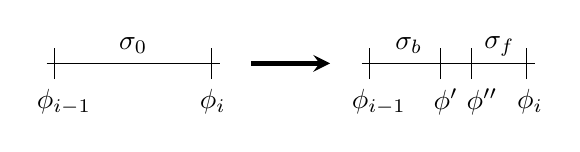
\begin{tikzpicture}
        \draw (-5.1, 0) -- (-2.9, 0);
        \draw (-5, -.2) -- (-5, .2);
        \draw (-3, -.2) -- (-3, .2);
        \node [below] at (-4.88, -.2) {$\phi_{i-1}$};
        \node [below] at (-2.99, -.2) {$\phi_i$};
        \node [above] at (-4, 0) {$\sigma_0$};

        \draw [ultra thick,->,>=stealth] (-2.5, 0) -- (-1.5, 0);

        \draw (-1.1, 0) -- (1.1, 0);
        \draw (-1, -.2) -- (-1, .2);
        \draw (1, -.2) -- (1, .2);
        \draw (.3, -.2) -- (.3, .2);
        \draw (-.1, -.2) -- (-.1, .2);
        \node [below] at (-.88, -.2) {$\phi_{i-1}$};
        \node [below] at (1.04, -.2) {$\phi_i$};
        \node [below] at (.43, -.2) {$\phi''$};
        \node [below] at (-.03, -.2) {$\phi'$};
        \node [above] at (.65, -.04) {$\sigma_f$};
        \node [above] at (-.5, 0) {$\sigma_b$};
    \end{tikzpicture}
    \caption{Diagram of the addition of two LNCs}
    \label{fig:lnc_diagram}
\end{figure}

We then put an angular restriction on the two new linking number constraints. By subtracting off the excess angle \(\phi\) that the undisturbed DNA has prior to RNAP binding (linearly interpolated because we assume complete supercoiling relaxing), we can define:
\begin{equation}
    \Delta \phi' = \phi' - \left(\phi_{i - 1} + \frac{z' - z_{i-1}}{z_i - z_{i-1}} (\phi_i - \phi_{i-1})\right)
\end{equation}

\begin{equation}
    \Delta \phi'' = \phi'' - \left(\phi_{i - 1} + \frac{z'' - z_{i-1}}{z_i - z_{i-1}} (\phi_i - \phi_{i-1})\right)
\end{equation}

For unwinding of the region bound to the RNAP to occur, we impose two constraints:
\begin{equation}
    |\Delta \phi'| + |\Delta \phi''| = 1.2 \cdot 2 \pi
\end{equation}
\begin{equation}
    \Delta \phi' - \Delta \phi'' = 1.2 \cdot 2\pi
\end{equation}
In words, for the middle region, two different ways to unwind it would either to rotate the leading LNC backwards or rotate the trailing LNC forwards. There are also many intermediate solutions where \emph{both} of the bounding LNCs move. The first restriction is there to ensure that we use the solution that minimizes total amount of rotation needed.

Given a complete energy model, minimizing the energy cost with respect to \(\Delta \phi'\) or \(\Delta \phi''\) could give a unique solution for any one specific geometry.

\subsubsection{Order of magnitude analysis of induced change in supercoiling}
How much does inducing these rotations change the supercoiling density in each of the three regions of interest?

Using our definition in \autoref{eq:sc_density}, perturbing the RNAP bound region introduces a change in supercoiling of:
\begin{equation}
    \Delta \sigma_\text{RNAP} = \frac{\Delta \phi'' - \Delta \phi'}{\omega_0 |13 \text{bp}|} = \frac{-1.2 \cdot 2\pi}{\omega_0 \cdot 4.42 \text{nm}} = -0.92
    \label{eq:delta_sigma_rnap}
\end{equation}
This is a very large change in supercoiling density! This is expected, as complete melting/unwinding of the RNAP-bound region is a very large perturbation. In contrast, the change in supercoiling density either behind or forward of the RNAP is much smaller, and depends on the size of the leading or following region:

\begin{equation}
\Delta \sigma_b = \frac{1.2 \cdot 2 \pi}{\omega_0 |z' - z_{i-1}|}
\end{equation}
A 600 bp region (204 nm) is sufficient to reduce \(\Delta \sigma_b \sim 0.02\), even in the worst case scenario where \(\Delta \phi' = 1.2 \cdot 2  \pi, \Delta \phi'' = 0\).

In practice, this worst case should only happen when \(\phi_{i-1}\) and \(\phi_i\) are separated by around this distance, and the RNAP binds right by one of the edges.

\subsubsection{Model formulation: external supercoiling}
We now need to find the energetic change of RNAP binding as a function of \(\sigma_0\), the initial supercoiling rate.

We could do this in one of two ways; if we knew the torque response at each new LNC, averaged over the unwinding event, we could calculate it directly as
\begin{equation}
    \Delta E = \overline \tau' \Delta \phi' + \overline \tau'' \Delta \phi''
    \label{eq:direct_torque_calc}
\end{equation}

If we assume that the energy surface is locally linear, then we can relate the instantaneous torque to the change in energy. Marko defines:
\[ \tau = \frac{1}{\omega_0} \frac{\partial S(\sigma)}{\partial \sigma}\]
for \(S\) the energy per unit length. This means that:
\begin{equation}
    \Delta E = (z_2 - z_1) \tau \omega_0 \Delta \sigma = (z_2 - z_1) \frac{\partial S}{\partial \sigma} \Delta \sigma
\end{equation}
By expanding the definition of \(\Delta \sigma\) for an arbitrary region bounded by LNC1 and LNC2 under this locally linear assumption, we can actually recover the normal energy-torque definition:
\[\Delta E = (z_2 - z_1) \tau \omega_0 \frac{\Delta\phi_2 - \Delta\phi_1}{\omega_0 (z_2 - z_1)} = \tau (\Delta \phi_2 - \Delta\phi_1)\]
Note that this implies that the energy cost of LNC rotation is independent of the region width; under a locally linear assumption, the energy cost depends only on the local instantaneous torque and the rotation angle.

Looking at the free energy surface as a function of supercoiling in \autoref{fig:marko_energy_surface}, we see that a locally linear approximation should be relatively valid in the  ``exterior'' regions, but will be very incorrect if we apply this approximation for the RNAP-bound interior region where complete melting occurs.

\begin{figure}[h]
    \centering
    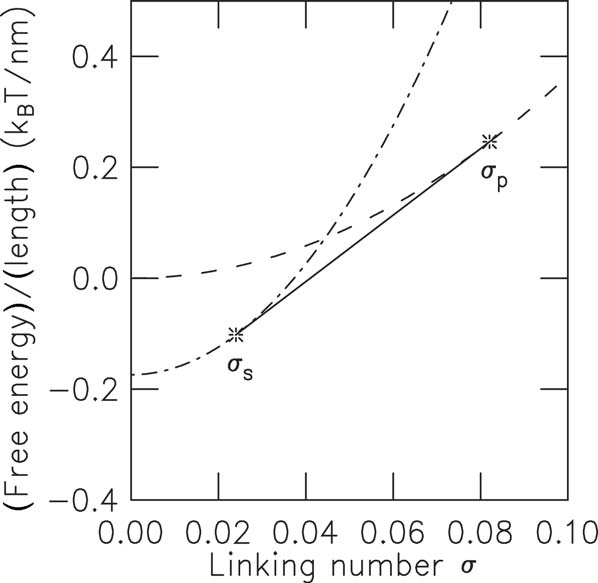
\includegraphics[width=.5\linewidth]{figures/marko_linking_number_graph}
    \caption{Plot of an example energy surface. Reproduced Figure 1 from \textcite{markoTorqueDynamicsLinking2007}.}
    \label{fig:marko_energy_surface}
\end{figure}
\subsubsection{Model formulation: internal melting}
Our model derives energy differences based on the difference between the (assumed to be locally linear) energy cost of increasing supercoiling in the exterior regions,
versus the integrated energy difference in the interior region. This means we model:
\[\Delta E = \tau(\sigma_0) \cdot 1.2 \cdot 2\pi + \int_{\sigma_0}^{\sigma_0 + \Delta \sigma_\text{RNAP}} \Delta z_\text{RNAP} \frac{\partial S}{\partial \sigma} d\sigma\]
for \(\Delta z_\text{RNAP} = 13 \text{bp} = 4.42 \text{nm}\) and \(\Delta \sigma_\text{RNAP} = -0.92\) as in \autoref{eq:delta_sigma_rnap}.

Given the well-defined structure of the RNAP-DNA complex and the fact that under all realistic physiological conditions \(\Delta \sigma_\text{RNAP} \gg \sigma_0\), we assume that the end-state energy is a constant, but unknown \(S_\text{unwound}\):
\begin{equation}
    \Delta E = \tau(\sigma_0) \cdot 1.2 \cdot 2\pi + \Delta z_\text{RNAP} \left(S_\text{unwound} - S(\omega_0)\right)
\end{equation}


However, when we compare the strength of this internal melting energy term to the ``exterior'' supercoiling term, we see that the external term dominates (\autoref{fig:app:energy_comparison}).
\begin{figure}[h]
    \centering
    %\includegraphics[width=.5\linewidth]{figures/energy_plot}
    \caption{Plotted is the binding energy required to bind an RNAP, for different starting values of \(\sigma_0\). In the single-phase regions, differences in \(\Delta E\) are dominated by the external torque term. In the two-phase region, \(\Delta E\) remains mostly constant!}
    \label{fig:app:energy_comparison}
\end{figure}
which means we can use the simple form:
\begin{equation}
    \Delta E = \tau(\sigma_0) \cdot 1.2 \cdot 2\pi
\end{equation}


\FloatBarrier
\subsubsection{Model evaluation}
This equation has some of the features that we wanted in the model. Consider the change in \(\Delta E\) by a \(\Delta \sigma\) change in the coexistence region where:
\[\tau = \frac{1}{\omega_0} \sqrt{2pg}{1 - \frac{p}{c_s}} = \text{constant}\]
\[S = \frac{-g}{1 - \frac{p}{c_s}} + \sqrt{\frac{2pg}{1 - \frac{p}{c_s}}} \sigma\]
for \(\sigma_2 = \sigma_1 + \Delta \sigma\). Then,
\[\Delta E_2 - \Delta E_1 = - \Delta z_\text{RNAP} \left( \frac{-g}{1 - \frac{p}{c_s}} + \sqrt{\frac{2pg}{1-\frac{p}{c_s}}} \Delta \sigma\right)\]

This means that we do not have a strictly constant binding energy in the constant-torque region. However, if we plot the value of \(\Delta E\) across various supercoiling values, for the mean value of constants given in \autoref{tab:constants}, we see that the unwinding energy does remain relatively constant in the constant torque regime!

The values for \(\Delta E\) are much larger than initially expected; Literature results show that the RNAP on-rate decreases roughly four-fold in the first single-phase region, which occurs for \(\Delta E \sim 4 \text{pN nm}\).

This discrepancy means that we expect our initial supercoiling-initiation model to be a useful way to upper-bound the effects of this behavior on the system. Realistically, secondary chromatin effects such as nucleosome displacement may allow for the high energy cost of adding polymerases to already supercoiled regions to be diminished.

\begin{figure}[h]
    \centering
    \begin{subfigure}{.49\linewidth}
        \centering
%        \includegraphics[width=.99\textwidth]{figures/time_plot}
        \caption{Plot of the inverse RNAP on-rate, as modeled here.}
    \end{subfigure}
    \begin{subfigure}{.49\linewidth}
        \centering
        %\includegraphics[width=.8\textwidth]{figures/revyakin_plot}
        \caption{Reproduced Figure 3c from \textcite{revyakinPromoterUnwindingPromoter2004}.}
    \end{subfigure}
    \caption{Our model predictions appear to replicate literature results. Even though \(\Delta E\) is not strictly constant in the two-phase/constant-torque region, its numerical value is nearly constant in that region.}
\end{figure}
\end{document}
